\setbackground
{
	\centering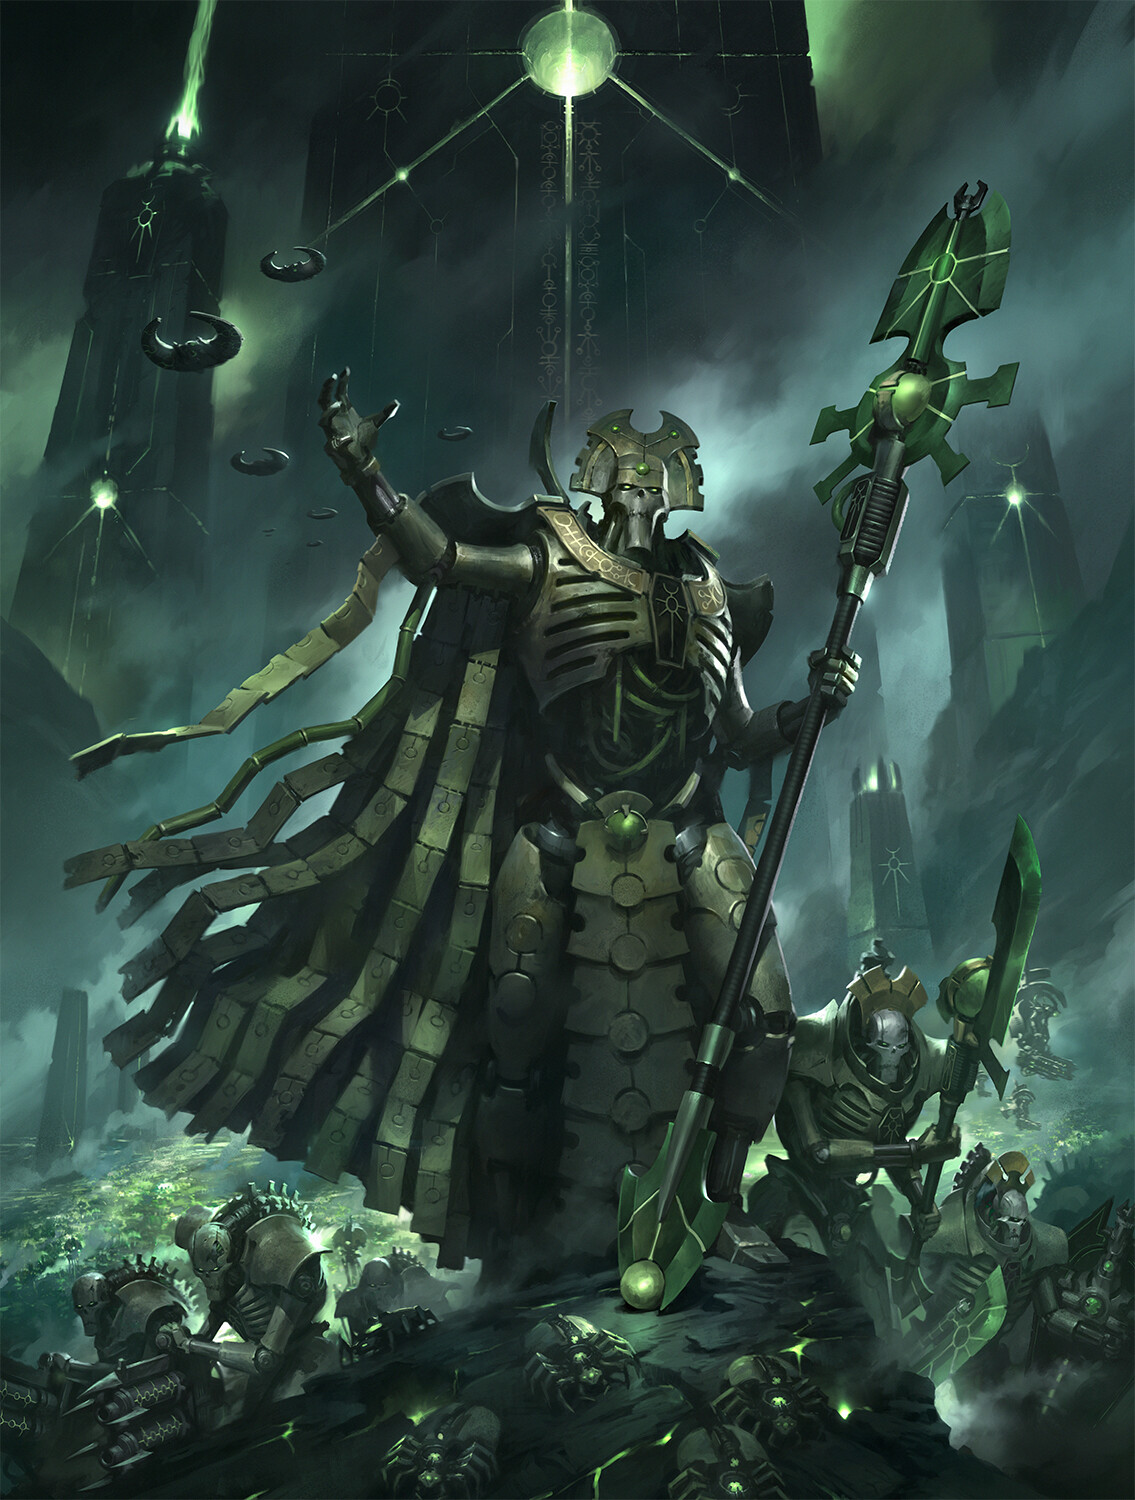
\includegraphics[height=530pt, width=400pt]{hq_art.jpg}
	\subsection{\texorpdfstring{\centering\Huge HQ}{HQ}}
	
	\centerline{\begin{minipage}{400pt}
			\centering
			'You stupid bastard, you got us box seats to a coup.’
			
			‘Well, the reviews were very good.'
			
			\vspace*{1em}
			\raggedleft Orikan the Diviner to Trazyn the Infinite
	\end{minipage}}
}

\newpage
\clearbackground
\subsubsection[Lord]{}

\fbox{\begin{imgminipage}{marble.jpg}[t]{0.2\textwidth}
		\color{white}
		\centering {\large HQ}
		
		\raggedright \small
		\color{black}
\end{imgminipage}}
\hspace{0.5em}
\begin{minipage}[t]{0.72\textwidth}
	{\large \textbf{Lord \dotfill 40 Points}}
	
	\begin{tabular}{m{165 pt} *{10}{c}}
		& M & WS & BS & S & T & W & I & A & Ld & Sv \\
		\hline
		Lord & 7 & 4 & 4 & 5 & 5 & 2 & 2 & 2 & 10 & 3+ \\
	\end{tabular}
	\small
	\begin{minipage}[t]{0.5\textwidth}
		\begin{flushleft}
		\vspace*{2em}
		\textbf{Unit Composition}
		\begin{itemize}
			\item 1 Lord
		\end{itemize}
		
		\textbf{Wargear}
		\begin{itemize}
			\item \quickref{Staff of Light}
		\end{itemize}
		\end{flushleft}
	\end{minipage}
	\begin{minipage}[t]{0.5\textwidth}
		\begin{flushleft}
		\vspace*{2em}
		\textbf{Unit Type}
		\begin{itemize}
			\item Infantry (Character, \quickref{Living Metal}, \quickref{Noble})
		\end{itemize}
		
		\textbf{Special Rules}
		\begin{itemize}
			\item \quickref{Command Protocols}
			\item \quickref{Nodal Command} (Bronze)
			\item \quickref{Reanimation Protocols}
			\item Relentless
		\end{itemize}
		\end{flushleft}
	\end{minipage}
	
	\vspace*{2em}
	\textbf{Weapons}
	
	\begin{tabular}{m{95 pt} *{4}{c} >{\raggedright\arraybackslash}p{130pt}}
		& Range & Type & S & AP & Abilities \\
		\hline
		\quickref{Staff of Light} & & &  &  &  \\
		— Shooting & 18" & Assault 3 & 5 & 3 & — \\
		— Melee & — & Melee & User & 3 & Rending (6+) \\
		\quickref{Hyperphase Sword} & — & Melee & User & 3 & Rending (5+) \\
		\quickref{Voidblade} & — & Melee & User & 4 & \quickref{Entropic Strike} (4+), Rending(6+) \\
		\quickref{Warscythe} & — & Melee & +2 & 2 & Armourbane (Melee), Two-Handed \\
		\quickref{Relic Gauss Blaster} & 30" & Rapid Fire 2 & 5 & 4 & \quickref{Gauss} (6+), Master-Crafted \\
	\end{tabular}
	
	\vspace*{2em}
	\textbf{Options}
	\begin{itemize}
		\item The Lord may exchange their \quickref{Staff of Light} for one of the following options:
		\begin{itemize}			
			\item \quickref{Hyperphase Sword} \dotfill -2 points
			\item \quickref{Voidblade} \dotfill +0 points
			\item \quickref{Warscythe} \dotfill +20 points
			\item \quickref{Warscythe} with in-built \quickref{Relic Gauss Blaster} \dotfill +30 points
		\end{itemize}
		\item The Lord may take any of the following options:
		\begin{itemize}
			\item \quickref{Gauntlet of Fire} \dotfill +10 points
			\item \quickref{Tachyon Arrow} \dotfill +150 points
			\item \quickref{Mindshackle Scarabs} \dotfill +20 points
			\item \quickref{Phase Shifter} \dotfill +25 points
			\item \quickref{Phylactery} \dotfill +10 points
			\item \quickref{Resurrection Orb} \dotfill +25 points
			\item \quickref{Translocation Shroud} \dotfill +10 points
		\end{itemize}
		\item The Lord may take equipment from the \quickref{Artefacts of the Aeons} list.
	\end{itemize}
\end{minipage}



\newpage
\subsubsection[Nemesor Lord]{}

\begin{minipage}[t]{0.72\textwidth}
	{\large \textbf{Nemesor Lord \dotfill 65 points}}
	
	\begin{tabular}{m{165 pt} *{10}{c}}
		& M & WS & BS & S & T & W & I & A & Ld & Sv \\
		\hline
		Nemesor Lord & 7 & 5 & 4 & 5 & 5 & 3 & 2 & 3 & 10 & 3+ \\
	\end{tabular}
	\small
	\begin{minipage}[t]{0.5\textwidth}
		\begin{flushleft}
		\vspace*{2em}
		\textbf{Unit Composition}
		\begin{itemize}
			\item 1 Nemesor Lord
		\end{itemize}
		
		\textbf{Wargear}
		\begin{itemize}
			\item \quickref{Staff of Light}
		\end{itemize}
		\end{flushleft}
	\end{minipage}
	\begin{minipage}[t]{0.5\textwidth}
		\begin{flushleft}
		\vspace*{2em}
		\textbf{Unit Type}
		\begin{itemize}
			\item Infantry (Character, \quickref{Living Metal}, \quickref{Noble})
		\end{itemize}
		
		\textbf{Special Rules}
		\begin{itemize}
			\item \quickref{Command Protocols}
			\item \quickref{Decurion Nemesor}
			\item \quickref{Nodal Command} (Silver)
			\item \quickref{Reanimation Protocols}
			\item Relentless
		\end{itemize}
		\end{flushleft}
	\end{minipage}
	
	\vspace*{2em}
	\textbf{Weapons}
	
	\begin{tabular}{m{95 pt} *{4}{c} >{\raggedright\arraybackslash}p{130pt}}
		& Range & Type & S & AP & Abilities \\
		\hline
		\quickref{Staff of Light} & & &  &  &  \\
		— Shooting & 18" & Assault 3 & 5 & 3 & — \\
		— Melee & — & Melee & User & 3 & Rending (6+) \\
		\quickref{Hyperphase Sword} & — & Melee & User & 3 & Rending (5+) \\
		\quickref{Voidblade} & — & Melee & User & 4 & \quickref{Entropic Strike} (4+), Rending(6+) \\
		\quickref{Warscythe} & — & Melee & +2 & 2 & Armourbane (Melee), Two-Handed \\
		\quickref{Relic Gauss Blaster} & 30" & Rapid Fire 2 & 5 & 4 & \quickref{Gauss} (6+), Master-Crafted \\
		\quickref{Rod of Night} & & &  &  &  \\
		— Shooting & 18" & Assault 2 & 5 & — & Haywire, \quickref{Tesla} (6+) \\
		— Melee & — & Melee & User & — & \quickref{Energy Siphon}, Haywire \\
	\end{tabular}
	
	\vspace*{2em}
	\textbf{Dedicated Transport}
	A Nemesor Lord may take a Catacomb Command Barge as a Dedicated Transport. As a Dedicated Transport this does not use up an additional Force Organisation slot, but its points cost must still be paid for as part of the army.
	
	\vspace*{2em}
	\textbf{Options}
	\begin{itemize}
		\item The Nemesor Lord may exchange their \quickref{Staff of Light} for one of the following options:
		\begin{itemize}			
			\item \quickref{Hyperphase Sword} \dotfill -2 points
			\item \quickref{Rod of Night} \dotfill +5 points
			\item \quickref{Voidblade} \dotfill +0 points
			\item \quickref{Warscythe} \dotfill +20 points
			\item \quickref{Warscythe} with in-built \quickref{Relic Gauss Blaster} \dotfill +30 points
		\end{itemize}
		\item A Nemesor Lord without a Two-Handed weapon may take the following:
		\begin{itemize}
			\item \quickref{Dispersion Shield} \dotfill +30 points
		\end{itemize}
		\item The Nemesor Lord may take any of the following options:
		\begin{itemize}
			\item \quickref{Gauntlet of Fire} \dotfill +10 points
			\item \quickref{Tachyon Arrow} \dotfill +150 points
			\item \quickref{Mindshackle Scarabs} \dotfill +20 points
			\item \quickref{Phase Shifter} \dotfill +25 points
			\item \quickref{Phylactery} \dotfill +10 points
			\item \quickref{Resurrection Orb} \dotfill +25 points
			\item \quickref{Sempiternal Weave} \dotfill +10 points
			\item \quickref{Tesseract Labyrinth} \dotfill +100 points
			\item \quickref{Translocation Shroud} \dotfill +10 points
		\end{itemize}
		\item The Nemesor Lord may take equipment from the \quickref{Artefacts of the Aeons} list.
	\end{itemize}
\end{minipage}
\hspace{0.5em}
\fbox{\begin{imgminipage}{marble.jpg}[t]{0.2\textwidth}
	\color{white}
	\centering {\large HQ}
	
	\raggedleft \small
	\color{black}
\end{imgminipage}}



\newpage
\subsubsection[Nemesor Overlord]{}

\fbox{\begin{imgminipage}{marble.jpg}[t]{0.2\textwidth}
		\color{white}
		\centering {\large HQ}
		
		\raggedright \small
		\color{black}
\end{imgminipage}}
\hspace{0.5em}
\begin{minipage}[t]{0.72\textwidth}
	{\large \textbf{Nemesor Overlord \dotfill 85 points}}
	
	\begin{tabular}{m{165 pt} *{10}{c}}
		& M & WS & BS & S & T & W & I & A & Ld & Sv \\
		\hline
		Nemesor Overlord & 7 & 5 & 5 & 5 & 5 & 4 & 2 & 3 & 10 & 3+ \\
	\end{tabular}
	\small
	\begin{minipage}[t]{0.5\textwidth}
		\begin{flushleft}
		\vspace*{2em}
		\textbf{Unit Composition}
		\begin{itemize}
			\item 1 Nemesor Overlord
		\end{itemize}
		
		\textbf{Wargear}
		\begin{itemize}
			\item \quickref{Staff of Light}
		\end{itemize}
		\end{flushleft}
	\end{minipage}
	\begin{minipage}[t]{0.5\textwidth}
		\begin{flushleft}
		\vspace*{2em}
		\textbf{Unit Type}
		\begin{itemize}
			\item Infantry (Character, \quickref{Living Metal}, \quickref{Noble})
		\end{itemize}
		
		\textbf{Special Rules}
		\begin{itemize}
			\item \quickref{Command Protocols}
			\item My Will Be Done
			\item \quickref{Nodal Command} (Gold)
			\item Overlord's Court
			\item \quickref{Reanimation Protocols}
			\item Relentless
			\item \quickref{Tesserarion Nemesor}
		\end{itemize}
		\end{flushleft}
	\end{minipage}
		
	\vspace*{2em}
	\textbf{Weapons}
	
	\begin{tabular}{m{95 pt} *{4}{c} >{\raggedright\arraybackslash}p{130pt}}
		& Range & Type & S & AP & Abilities \\
		\hline
		\quickref{Staff of Light} & & &  &  &  \\
		— Shooting & 18" & Assault 3 & 5 & 3 & — \\
		— Melee & — & Melee & User & 3 & Rending (6+) \\
		\quickref{Hyperphase Sword} & — & Melee & User & 3 & Rending (5+) \\
		\quickref{Voidblade} & — & Melee & User & 4 & \quickref{Entropic Strike} (4+), Rending(6+) \\
		\quickref{Voidscythe} & — & Melee & x2 & 1 & \quickref{Entropic Strike} (2+), Brutal (2), Unwieldy, Two-Handed \\
		\quickref{Warscythe} & — & Melee & +2 & 2 & Armourbane (Melee), Two-Handed \\
		\quickref{Relic Gauss Blaster} & 30" & Rapid Fire 2 & 5 & 4 & \quickref{Gauss} (6+), Master-Crafted \\
		\quickref{Rod of Night} & & &  &  &  \\
		— Shooting & 18" & Assault 2 & 5 & — & Haywire, \quickref{Tesla} (6+) \\
		— Melee & — & Melee & User & — & \quickref{Energy Siphon}, Haywire \\
	\end{tabular}
	
	\vspace*{2em}
	\textbf{Unit Rules}
	
	\textit{My Will Be Done:} A Nemesor Overlord automatically passes all Command Protocol checks.
	
	\textit{Overlord's Court:} When taking a Nemesor Overlord, you may also take one additional Lord or Nemesor Lord without using up an additional Force Organization Slot. 
	
	\vspace*{2em}
	\textbf{Dedicated Transport}
	A Nemesor Overlord may take a Catacomb Command Barge as a Dedicated Transport. As a Dedicated Transport this does not use up an additional Force Organisation slot, but its points cost must still be paid for as part of the army.
	
	\vspace*{2em}
	\textbf{Options}
	\begin{itemize}
		\item The Nemesor Overlord may exchange their \quickref{Staff of Light} for one of the following options:
		\begin{itemize}			
			\item \quickref{Hyperphase Sword} \dotfill -2 points
			\item \quickref{Rod of Night} \dotfill +5 points
			\item \quickref{Voidblade} \dotfill +0 points
			\item \quickref{Warscythe} \dotfill +20 points
			\item \quickref{Warscythe} with in-built \quickref{Relic Gauss Blaster} \dotfill +30 points
		\end{itemize}
		\item A Nemesor Overlord without a Two-Handed weapon may take the following:
		\begin{itemize}
			\item \quickref{Dispersion Shield} \dotfill +30 points
		\end{itemize}
		\item The Nemesor Overlord may take any of the following options:
		\begin{itemize}
			\item \quickref{Gauntlet of Fire} \dotfill +10 points
			\item \quickref{Tachyon Arrow} \dotfill +1+0 points
			\item \quickref{Mindshackle Scarabs} \dotfill +20 points
			\item \quickref{Phase Shifter} \dotfill +25 points
			\item \quickref{Phylactery} \dotfill +10 points
			\item \quickref{Resurrection Orb} \dotfill +25 points
			\item \quickref{Sempiternal Weave} \dotfill +10 points
			\item \quickref{Shadow Ankh} \dotfill +10 points
			\item \quickref{Tesseract Labyrinth} \dotfill +100 points
			\item \quickref{Translocation Shroud} \dotfill +10 points
		\end{itemize}
		\item The Nemesor Overlord may take equipment from the \quickref{Artefacts of the Aeons} list.
	\end{itemize}
\end{minipage}


\newpage
\subsubsection[Phaeron]{}

\begin{minipage}[t]{0.72\textwidth}
	{\large \textbf{Phaeron \dotfill X points}}
	
	\begin{tabular}{m{165 pt} *{10}{c}}
		& M & WS & BS & S & T & W & I & A & Ld & Sv \\
		\hline
		Phaeron & 7 & 6 & 6 & 5 & 5 & 4 & 2 & 4 & 10 & 3+ \\
	\end{tabular}
	\small
	\begin{minipage}[t]{0.5\textwidth}
		\begin{flushleft}
		\vspace*{2em}
		\textbf{Unit Composition}
		\begin{itemize}
			\item 1 Phaeron
		\end{itemize}
		
		\textbf{Wargear}
		\begin{itemize}
			\item \quickref{Staff of Light}
		\end{itemize}
		\end{flushleft}
	\end{minipage}
	\begin{minipage}[t]{0.5\textwidth}
		\begin{flushleft}
		\vspace*{2em}
		\textbf{Unit Type}
		\begin{itemize}
			\item Infantry (Character, \quickref{Living Metal}, \quickref{Noble}, \quickref{Phaeron}, Unique)
		\end{itemize}
		
		\textbf{Special Rules}
		\begin{itemize}
			\item \quickref{Command Protocols}
			\item My Will Be Done
			\item \quickref{Nodal Command} (Platinum)
			\item Phaeron's Court
			\item \quickref{Reanimation Protocols}
			\item \quickref{Tesserarion Nemesor}
		\end{itemize}
		\end{flushleft}
	\end{minipage}
	
	\vspace*{2em}
	\textbf{Weapons}
	
	\begin{tabular}{m{95 pt} *{4}{c} >{\raggedright\arraybackslash}p{130pt}}
		& Range & Type & S & AP & Abilities \\
		\hline
		\quickref{Staff of Light} & & &  &  &  \\
		— Shooting & 18" & Assault 3 & 5 & 3 & — \\
		— Melee & — & Melee & User & 3 & Rending (6+) \\
		\quickref{Hyperphase Sword} & — & Melee & User & 3 & Rending (5+) \\
		\quickref{Voidblade} & — & Melee & User & 4 & \quickref{Entropic Strike} (4+), Rending(6+) \\
		\quickref{Voidscythe} & — & Melee & x2 & 1 & \quickref{Entropic Strike} (2+), Brutal (2), Unwieldy, Two-Handed \\
		\quickref{Warscythe} & — & Melee & +2 & 2 & Armourbane (Melee), Two-Handed \\
		\quickref{Relic Gauss Blaster} & 30" & Rapid Fire 2 & 5 & 4 & \quickref{Gauss} (6+), Master-Crafted \\
		\quickref{Rod of Night} & & &  &  &  \\
		— Shooting & 18" & Assault 2 & 5 & — & Haywire, \quickref{Tesla} (6+) \\
		— Melee & — & Melee & User & — & \quickref{Energy Siphon}, Haywire \\
	\end{tabular}
	
	\vspace*{2em}
	\textbf{Unit Rules}
	
	\textit{My Will Be Done:} A Phaeron automatically passes all Command Protocol checks.
	
	\textit{Phaeron's Court:} When taking a Phaeron, you may also take up to 2 Nemesor Overlords without using up an additional Force Organization Slot. 
	
	\vspace*{2em}
	\textbf{Dedicated Transport}
	A Phaeron may take a Catacomb Command Barge as a Dedicated Transport. As a Dedicated Transport this does not use up an additional Force Organisation slot, but its points cost must still be paid for as part of the army.
	
	\vspace*{2em}
	\textbf{Options}
	\begin{itemize}
		\item The Phaeron may exchange their \quickref{Staff of Light} for one of the following options:
		\begin{itemize}			
			\item \quickref{Hyperphase Sword} \dotfill -2 points
			\item \quickref{Rod of Night} \dotfill +5 points
			\item \quickref{Voidblade} \dotfill +0 points
			\item \quickref{Warscythe} \dotfill +20 points
			\item \quickref{Warscythe} with in-built \quickref{Relic Gauss Blaster} \dotfill +30 points
		\end{itemize}
		\item A Phaeron without a Two-Handed weapon may take the following:
		\begin{itemize}
			\item \quickref{Dispersion Shield} \dotfill +30 points
		\end{itemize}
		\item The Phaeron may take any of the following options:
		\begin{itemize}
			\item \quickref{Gauntlet of Fire} \dotfill +10 points
			\item \quickref{Tachyon Arrow} \dotfill +190 points
			\item \quickref{Mindshackle Scarabs} \dotfill +20 points
			\item \quickref{Phase Shifter} \dotfill +25 points
			\item \quickref{Phylactery} \dotfill +10 points
			\item \quickref{Resurrection Orb} \dotfill +25 points
			\item \quickref{Sempiternal Weave} \dotfill +10 points
			\item \quickref{Shadow Ankh} \dotfill +10 points
			\item \quickref{Tesseract Labyrinth} \dotfill +100 points
			\item \quickref{Translocation Shroud} \dotfill +10 points
		\end{itemize}
		\item The Phaeron may take equipment from the \quickref{Artefacts of the Aeons} list.
	\end{itemize}
\end{minipage}
\hspace{0.5em}
\fbox{\begin{imgminipage}{marble.jpg}[t]{0.2\textwidth}
		\color{white}
		\centering {\large PHAERON}
		
		\raggedleft \small
		\color{black}
\end{imgminipage}}

\newpage
\subsubsection[Catacomb Command Barge]{}
\fbox{\begin{imgminipage}{marble.jpg}[t]{0.2\textwidth}
		\color{white}
		\centering {\large HQ}
		
		\raggedright \small
		\color{black}
\end{imgminipage}}
\hspace{0.5em}
\begin{minipage}[t]{0.72\textwidth}
	{\large \textbf{Catacomb Command Barge \dotfill X Points}}
	\begin{NiceTabular}{m{145 pt} *{2}{c} | *{3}{c} | c | c }
		& & & \cellgray{3}{Armour} & & & & \cellgray{1}{Transport} \\
		& M & BS & \cellgray{1}{Front} & \cellgray{1}{Side} & \cellgray{1}{Rear} & HP & \cellgray{1}{Capacity} \\
		\hline
		Catacomb Command Barge & 12 & 4 & \cellgray{1}{11} & \cellgray{1}{11} & \cellgray{1}{11} & 3 &\cellgray{1}{1} \\
	\end{NiceTabular}
	\small
	\begin{minipage}[t]{0.5\textwidth}
		\begin{flushleft}
		\vspace*{2em}
		\textbf{Unit Composition}
		\begin{itemize}
			\item 1 Catacomb Command Barge
		\end{itemize}
		
		\textbf{Wargear}
		\begin{itemize}
			\item Hull (Front) Mounted \quickref{Gauss Cannon}
			\item \quickref{Quantum Shielding}
		\end{itemize}
		\end{flushleft}
	\end{minipage}
	\begin{minipage}[t]{0.5\textwidth}
		\begin{flushleft}
		\vspace*{2em}
		\textbf{Unit Type}
		\begin{itemize}
			\item Vehicle (Chariot, \quickref{Living Metal}, Open-Topped, Skimmer, Transport)
		\end{itemize}
		
		\textbf{Special Rules}
		\begin{itemize}
			\item Command Wave
		\end{itemize}
		\end{flushleft}
	\end{minipage}
	
	\vspace*{2em}
	\textbf{Access Points}
	
	The Catacomb Command Barge has one Access Point on each side of the hull.
	
	\vspace*{2em}
	\textbf{Weapons}
	
	\begin{tabular}{m{95 pt} *{4}{c} >{\raggedright\arraybackslash}p{130pt}}
		& Range & Type & S & AP & Abilities \\
		\hline
		\quickref{Gauss Cannon} & 24" & Heavy 3 & 6 & 3 & \quickref{Gauss} (6+) \\
		\quickref{Tesla Cannon} & 30" & Heavy 3 & 6 & — & \quickref{Tesla} (6+) \\
	\end{tabular}
	
	\vspace*{2em}
	\textbf{Unit Rules}
	
	\textit{Command Wave}: All friendly units with the Necrons Faction within \quickref{Nodal Range} of a Catacomb Command Barge re-roll all failed Morale, Pinning and Fear tests.
	
	\vspace*{2em}
	\textbf{Options}
	\begin{itemize}
		\item The Catacomb Command Barge may exchange its \quickref{Gauss Cannon} for a:
		\begin{itemize}
			\item \quickref{Tesla Cannon} \dotfill +X points
		\end{itemize}
		\item A Catacomb Command Barge may take:
		\begin{itemize}
			\item \quickref{Quantum Shielding Matrix} \dotfill X points
		\end{itemize} 
	\end{itemize}
\end{minipage}


\newpage

\newpage
\subsubsection[Royal Warden]{}
\begin{minipage}[t]{0.72\textwidth}
	{\large \textbf{Royal Warden \dotfill X Points}}
	
	\begin{tabular}{m{165 pt} *{10}{c}}
		& M & WS & BS & S & T & W & I & A & Ld & Sv \\
		\hline
		Royal Warden & 7 & 4 & 4 & 5 & 5 & 2 & 2 & 2 & 10 & 3+ \\
	\end{tabular}
	\small
	\begin{minipage}[t]{0.5\textwidth}
		\begin{flushleft}
		\vspace*{2em}
		\textbf{Unit Composition}
		\begin{itemize}
			\item 1 Royal Warden
		\end{itemize}
		
		\textbf{Wargear}
		\begin{itemize}
			\item Close Combat Weapon
			\item \quickref{Relic Gauss Blaster}
		\end{itemize}
		\end{flushleft}
	\end{minipage}
	\begin{minipage}{0.5\textwidth}
		\vspace*{2em}
		\textbf{Unit Type}
		\begin{itemize}
			\item Infantry (Character, \quickref{Living Metal})
		\end{itemize}
		
		\textbf{Special Rules}
		\begin{itemize}
			\item \quickref{Awakening Protocols} (Silver)
			\item Independent Character
			\item \quickref{Reanimation Protocols}
			\item %TODO: Some buff for being a lieutenant
		\end{itemize}
	\end{minipage}
	
	\vspace*{2em}
	\textbf{Weapons}
	
	\begin{tabular}{m{95 pt} *{4}{c} >{\raggedright\arraybackslash}p{130pt}}
		& Range & Type & S & AP & Abilities \\
		\hline
		\quickref{Relic Gauss Blaster} & 30" & Rapid Fire 2 & 5 & 4 & \quickref{Gauss} (6+), Master-Crafted \\
	\end{tabular}
\end{minipage}
\hspace{0.5em}
\fbox{\begin{imgminipage}{marble.jpg}[t]{0.2\textwidth}
		\color{white}
		\centering {\large HQ}
		
		\raggedleft \small
		\color{black}
\end{imgminipage}}



\newpage
\subsubsection[Vargard]{}

\fbox{\begin{imgminipage}{marble.jpg}[t]{0.2\textwidth}
		\color{white}
		\centering {\large HQ}
		
		\raggedright \small
		\color{black}
\end{imgminipage}}
\hspace{0.5em}
\begin{minipage}[t]{0.72\textwidth}
	{\large \textbf{Vargard \dotfill X Points}}
	
	\begin{tabular}{m{165 pt} *{10}{c}}
		& M & WS & BS & S & T & W & I & A & Ld & Sv \\
		\hline
		Vargard & 7 & 5 & 4 & 5 & 5 & 2 & 2 & 3 & 10 & 3+ \\
	\end{tabular}
	\small
	\begin{minipage}[t]{0.5\textwidth}
		\begin{flushleft}
		\vspace*{2em}
		\textbf{Unit Composition}
		\begin{itemize}
			\item 1 Vargard
		\end{itemize}
		
		\textbf{Wargear}
		\begin{itemize}
			\item \quickref{Warscythe}
		\end{itemize}
		\end{flushleft}
	\end{minipage}
	\begin{minipage}[t]{0.5\textwidth}
		\begin{flushleft}
		\vspace*{2em}
		\textbf{Unit Type}
		\begin{itemize}
			\item Infantry (Character, \quickref{Living Metal})
		\end{itemize}
		
		\textbf{Special Rules}
		\begin{itemize}
			\item \quickref{Awakening Protocols} (Silver)
			\item Independent Character
			\item Lord's Retainer
			\item \quickref{Reanimation Protocols}
		\end{itemize}
		\end{flushleft}
	\end{minipage}
	
	\vspace*{2em}
	\textbf{Weapons}
	
	\begin{tabular}{m{95 pt} *{4}{c} >{\raggedright\arraybackslash}p{130pt}}
		& Range & Type & S & AP & Abilities \\
		\hline
		\quickref{Hyperphase Sword} & — & Melee & User & 3 & Rending (5+) \\
		\quickref{Warscythe} & — & Melee & +2 & 2 & Armourbane (Melee), Two-Handed \\
		\quickref{Relic Gauss Blaster} & 30" & Rapid Fire 2 & 5 & 4 & \quickref{Gauss} (6+), Master-Crafted \\	
	\end{tabular}

	\vspace*{2em}
	\textbf{Unit Rules}
	
	\textit{Lord's Retainer:} If a unit contains a Vargard as well as one or more models with the Noble Unit Sub-type, any Wounds which would be allocated to the Noble (even those caused by the Precision Strikes (X) or Sniper special rules) may instead	be allocated to a Vargard first.

	\vspace*{2em}
	\textbf{Options}
	\begin{itemize}
		\item The Vargard may exchange their \quickref{Warscythe} for one of the following options:
		\begin{itemize}			
			\item \quickref{Hyperphase Sword} and \quickref{Dispersion Shield} \dotfill 10 points
			\item \quickref{Relic Gauss Blaster} \dotfill -10 points
			\item \quickref{Warscythe} with in-built \quickref{Relic Gauss Blaster} \dotfill 10 points
		\end{itemize}
		\item The Vargard may take any of the following options:
		\begin{itemize}
			\item \quickref{Phase Shifter} \dotfill +25 points
			\item \quickref{Phylactery} \dotfill +10 points
			\item \quickref{Sempiternal Weave} \dotfill +10 points
		\end{itemize}
	\end{itemize}
\end{minipage}


\newpage
\subsubsection[Cryptek Conclave]{}

\begin{minipage}[t]{0.72\textwidth}
	{\large \textbf{Cryptek Conclave \dotfill X Points}}
	
	\begin{tabular}{m{165 pt} *{10}{c}}
		& M & WS & BS & S & T & W & I & A & Ld & Sv \\
		\hline
		Cryptek & 6 & 4 & 4 & 4 & 4 & 2 & 2 & 1 & 10 & 4+ \\
		Cryptek Lord & 6 & 4 & 4 & 5 & 5 & 2 & 2 & 1 & 10 & 3+ \\
	\end{tabular}
	\small
	\begin{minipage}[t]{0.5\textwidth}
		\begin{flushleft}
		\vspace*{2em}
		\textbf{Unit Composition}
		\begin{itemize}
			\item 1 Cryptek
		\end{itemize}
		
		\textbf{Wargear}
		\begin{itemize}
			\item Dependent on Conclave
		\end{itemize}
		\end{flushleft}
	\end{minipage}
	\begin{minipage}[t]{0.5\textwidth}
		\begin{flushleft}
		\vspace*{2em}
		\textbf{Unit Type}
		\begin{itemize}
			\item Infantry (Character, \quickref{Living Metal})
		\end{itemize}
		
		\textbf{Special Rules}
		\begin{itemize}
			\item Arkane Command
			\item \quickref{Awakening Protocols} (Bronze)
			\item Conclave Discipline
			\item Dynastic Advisors
			\item Independent Character
			\item \quickref{Reanimation Protocols}
		\end{itemize}
		\end{flushleft}
	\end{minipage}
	
	\vspace*{2em}	
	\textbf{Unit Rules}
	
	\textit{Arkane Command:} Cryptek models have the \quickref{Nodal Command} (Bronze) special rule, while Cryptek Lord models have the \quickref{Nodal Command} (Silver) special rule. This rule does not satisfy the pre-requisites for their own unit's \quickref{Awakening Protocols}.
	
	\textit{Conclave Discipline:} When taking a Cryptek Conclave, you must select a \quickref{Cryptek Conclave Discipline} for the unit. When selecting wargear from Disciplines, each piece of \textit{optional} wargear may only be taken once per unit. Models with differing Disciplines may never be part of the same unit. Before the battle, each model may be split off from his unit and be assigned to lead a different unit.
	
	\textit{Dynastic Advisors:} A Cryptek Conclave may be taken with a Lord, Nemesor Lord, Nemesor Overlord, or Phaeron unit as part of its Royal Court without using up an additional Force Organisation slot. If you do so, the number of models in this unit cannot exceed 1 for Lords, 2 for Nemesor Lords, 4 for Nemesor Overlords, and 5 for Phaerons.
	
	\vspace*{2em}
	\textbf{Options}
	\begin{itemize}
		\item The Cryptek Conclave may include:
		\begin{itemize}
			\item Up to an additional 4 Crypteks \dotfill X points each
		\end{itemize}
		\item Up to one Cryptek may be upgraded to a:
		\begin{itemize}
			\item Cryptek Lord \dotfill +X Points
		\end{itemize}
		\item A Cryptek or Cryptek Lord may take any of the following options:
		\begin{itemize}
			\item \quickref{Mindshackle Scarabs} \dotfill +20 points
			\item \quickref{Phase Shifter} \dotfill +25 points
			\item \quickref{Phylactery} \dotfill +10 points
		\end{itemize}
		\item A Cryptek Lord may take any of the following options:
		\begin{itemize}
			\item \quickref{Sempiternal Weave} \dotfill +10 points
			\item \quickref{Tesseract Labyrinth} \dotfill +100 points
			\item \quickref{Translocation Shroud} \dotfill +10 points
		\end{itemize}
	\end{itemize}
\end{minipage}
\hspace{0.5em}
\fbox{\begin{imgminipage}{marble.jpg}[t]{0.2\textwidth}
		\color{white}
		\centering {\large HQ}
		
		\raggedright \small
		\color{black}
\end{imgminipage}}


\newpage
\subsection{Dramatis Personae}

\subsubsection{Anrakyr the Traveller}

\newpage
\subsubsection{Trazyn the Infinite}

\newpage
\subsubsection{Orikan the Diviner}

\newpage
\subsubsection{Szarekh, the Silent King}